\subsection{Experiment 4: Comparing Optimization Algorithms: RMSProp and SGD} \label{sec:exp4}

Experiment 4 tested two optimization algorithms on the generative models.

The experiment examined the performance of the RMSProp and \ac{SGD} optimizers, in contrast to the previous experiments that relied on the Adam optimizer.

This experiment utilized identical model architecture, loss function (\ac{BCE}), and dataset as Experiment 3. The code was transferred to \ac{LIACC} 1 hardware configuration, with minimal alterations.

The initial experiment in this set utilized the RMSProp optimizer's default settings. The comprehensive loss was $1.966$, comprising a generator loss of $0.558$ and a discriminator loss of $1.407$.

Figure~\ref{fig:exp4_rms_results} offers insight into the loss and last spectrogram produced during this trial.

The next experiment in the sequence employed the standard configuration of the \ac{SGD} optimizer (for specifics, see Section~\ref{sec:sgd}). The total loss was calculated to be $1.945$, with a generator loss of $0.516$ and a discriminator loss of $1.429$.

Figure~\ref{fig:exp4_sgd_results} presents the loss and the final spectrogram generated in this experiment.

The obtained results were comparable to those obtained with the Adam optimizer in previous iterations.

\begin{figure}[!ht]
    \centering
    \begin{subfigure}{0.45\textwidth}
        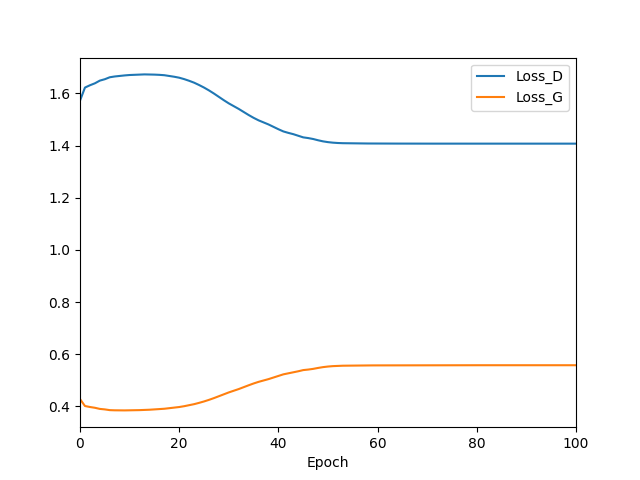
\includegraphics[width=\textwidth]{figures/4.5-results/exp4_rms_loss.png}
        \caption{Evolving losses throughout the training process for Experiment 4 with RMSprop.}
        \label{fig:exp4_rms_loss}
    \end{subfigure}
    \begin{subfigure}{0.45\textwidth}
        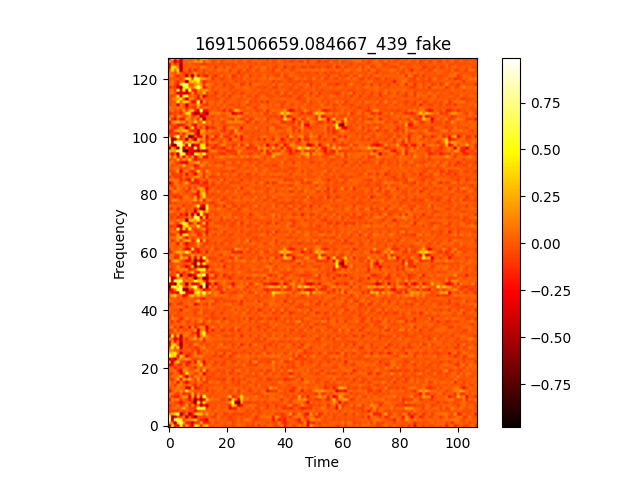
\includegraphics[width=\textwidth]{figures/4.5-results/exp4_rms_spectrogram.png}
        \caption{Spectrogram generated in Experiment 4 with RMSprop.}
        \label{fig:exp4_rms_spectrogram}
    \end{subfigure}
    \caption{Results of Experiment 4 with RMSprop.}
    \label{fig:exp4_rms_results}
\end{figure}

\begin{figure}[!ht]
    \centering
    \begin{subfigure}{0.45\textwidth}
        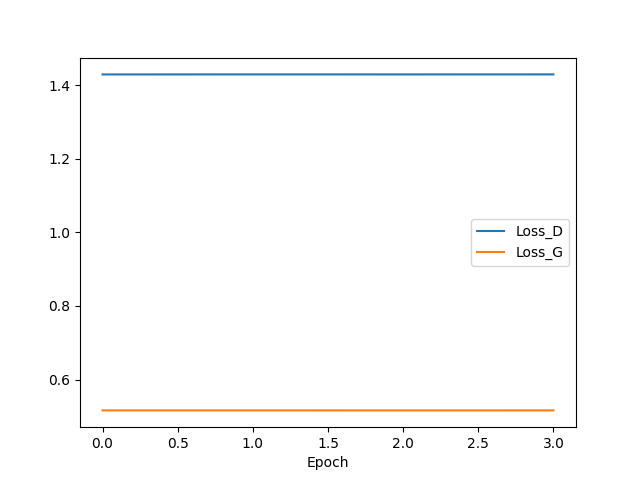
\includegraphics[width=\textwidth]{figures/4.5-results/exp4_sgd_loss.png}
        \caption{Evolving losses throughout the training process for Experiment 4 with \ac{SGD}.}
        \label{fig:exp4_sgd_loss}
    \end{subfigure}
    \begin{subfigure}{0.45\textwidth}
        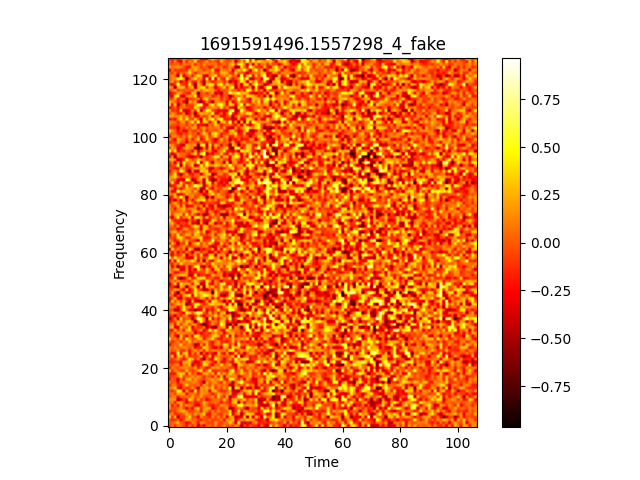
\includegraphics[width=\textwidth]{figures/4.5-results/exp4_sgd_spectrogram.png}
        \caption{Spectrogram generated in Experiment 4 with \ac{SGD}.}
        \label{fig:exp4_sgd_spectrogram}
    \end{subfigure}
    \caption{Results of Experiment 4 with \ac{SGD}.}
    \label{fig:exp4_sgd_results}
\end{figure}